\section{实验:测定物质的密度}\label{sec:4-2}

现在我们用实验来测定固体和液体的密度。为此需要测出它们的质量和体积,然后根据密度公式求出它们的密度。

质量可以用天平来测量。形状规则的物体,例如长方体,测出它的长、宽、高,就可以算出它的体积。


\begin{figure}[htbp]
    \centering
    \begin{minipage}{7cm}
    \centering
    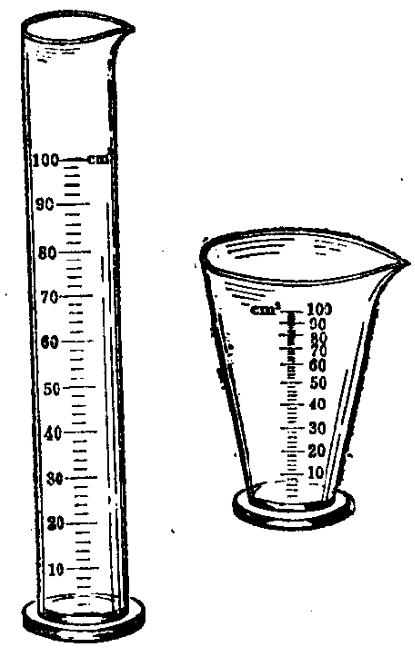
\includegraphics[width=4cm]{../pic/czwl1-ch4-3}
    \caption{}\label{fig:4-3}
    \end{minipage}
    \qquad
    \begin{minipage}{7cm}
    \centering
    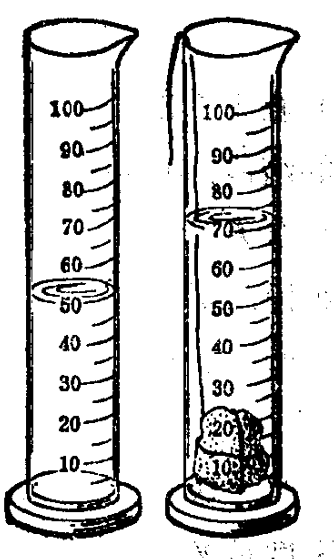
\includegraphics[width=4cm]{../pic/czwl1-ch4-4}
    \caption{}\label{fig:4-4}
    \end{minipage}
\end{figure}

液体的体积可以用量筒或量杯(图 \ref{fig:4-3})来测量。量筒和量杯的壁上有刻度,使用时要先弄清每小格代表多少立方厘米\footnotemark。
观察筒或杯里的液面到达的刻度,就可以知道液体的体积。用量筒或量杯还可以测量固体的体积。
测量时,先在筒或杯里倒入一定量的水,记下水面到达的刻度,然后把物体全部浸入水中。
再观察水面到达的刻度(图 \ref{fig:4-4}),从两次刻度的差就可以知道物体的体积。
\footnotetext{有的量筒或量杯的刻度是用毫升作单位的,$1 \text{亳升} = 1 \lflm$。}


观察量筒和量杯里水面到达的刻度时,视线要跟水面相平。量筒和量杯里的水面是凹形的,观察时要以凹形的底部为准。

\shiyan{目的} 用天平和量筒测定固体和液体的密度。

\shiyan{器材} 天平,砝码,量筒或量杯,铁块,玻璃杯,盐水,水,细线。

\shiyan{步骤}

(1) 用天平测出铁块的质量。

(2) 用量筒或量杯测出铁块的体积。

把 (1) (2) 中测得的数据填入表一中。
\begin{table}[H]
    \centering
    \caption*{\textbf{表一}}
    \begin{tabular}{|w{c}{6em}|w{c}{6em}|w{c}{8em}|w{c}{6em}|w{c}{6em}|}
        \hline
        \tabincell{c}{铁块的质量\\(克)} & \tabincell{c}{量筒内水\\的体积\\($\lflm$)} & \tabincell{c}{放入铁块后\\水面升到的刻度\\($\lflm$)} & \tabincell{c}{铁块的体积\\($\lflm$)} & \tabincell{c}{铁的密度\\($\kmlflm$)} \\ \hline
         & & & & \\ \hline
    \end{tabular}
\end{table}

(3) 用天平测出玻璃杯的质量。往玻璃杯里倒入适量的盐水,用天平测出玻璃杯和盐水的质量。

(4) 用量筒测出玻璃杯中盐水的体积。

把 (3) (4) 中测得的数据填入表二中。
\begin{table}[H]
    \centering
    \caption*{\textbf{表二}}
    \begin{tabular}{|w{c}{6em}|w{c}{8em}|w{c}{6em}|w{c}{6em}|w{c}{6em}|}
        \hline
        \tabincell{c}{玻璃杯的质量\\(克)} & \tabincell{c}{玻璃杯和\\盐水的质量\\(克)} & \tabincell{c}{盐水的质量\\(克)} & \tabincell{c}{盐水的体积\\($\lflm$)} & \tabincell{c}{盐水的密度\\($\kmlflm$)} \\ \hline
         & & & & \\ \hline
    \end{tabular}
\end{table}

\begin{wrapfigure}[8]{r}{3cm}
    \centering
    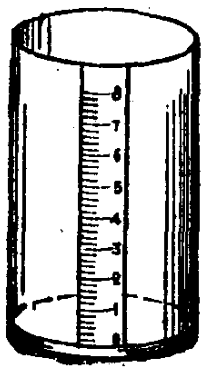
\includegraphics[width=2.5cm]{../pic/czwl1-ch4-5}
    \caption{}\label{fig:4-5}
\end{wrapfigure}


(5) 根据测得的数据分别求出铁和盐水的密度。

\shiyan{思考题} 想一想,如何用量筒测出不沉入水中的木块的体积?



\nonumsection{小制作:自制量筒}

用一个圆筒形的玻璃杯自制一个量筒。做法如下:用刻度尺量出杯的内径和杯的高度(高度取厘米的整数),算出杯的容积。
在杯的外壁上贴一张纸条( 图 \ref{fig:4-5})。把杯的高度按每厘米一格分成若干等份,画在纸条上。再把每等份分成五小格。
算出每小格代表的立方厘米数。这样,玻璃杯就成了一个量筒。

用自制的量筒测出牙膏皮(要除去残留的牙膏)的体积。用秤称出牙膏皮的质量,算出牙膏皮的密度。
查查密度表,看看这个牙膏皮是用什么金属做的。

